\chapter{General Introduction}

\section{The ocean, phytoplankton and why it matters}

The complexity of the ocean and its vast ecosystems has fascinated scientists to this day and most likely will continue to do so far into the future. Myriad life forms are embedded in a matrix so far removed from our mostly dry existence on top the earth’s crust. In the ocean, life moves in dilution, and the equivalents of forests and grasslands are hard to spot unless the concentration of tiny phytoplankton is so large, that deep blue turns into a milky green.

The term phytoplankton refers to microscopic marine photosynthetic organisms. These microorganisms form the basis of the oceanic food web and are primary producers of planetary scale, contributing roughly half of the oxygen in our atmosphere through photosynthesis \citep{Field2009}. Phytoplankton consists of mostly single-celled organisms, prokaryotes and eukaryotes from a highly diverse evolutionary background \citep{Falkowski2004a}. This large phylogenetic diversity is accompanied by a remarkable range of survival strategies, biogeochemical roles, shapes and sizes within the polyphyletic phytoplankton (see Figure \ref{FinkelPhySizeRange} for a size comparison). The emergence of such a large variety of organisms and the mechanisms sustaining their persistence has been one of the key questions in phytoplankton ecology over the last 50 years \citep{Hutchinson1961} % EST: elaborate on Hutchinson's paradox

\begin{figure}
\centering
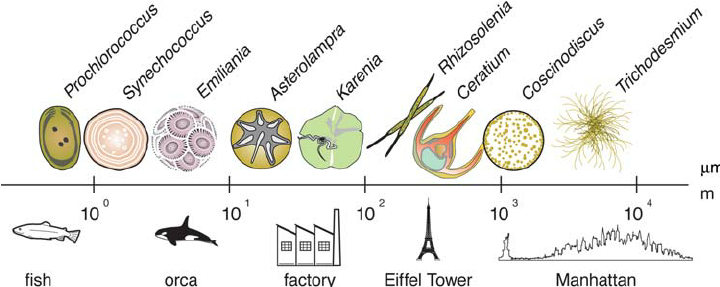
\includegraphics[trim = 0mm 0mm 0mm 0mm, clip, width=.9\linewidth]{./Chp1-Intro/SIZEphytoComparison_FinkelEtAl2010.png}
\caption[Scheme]{{\small "A comparison of the size range (maximum linear dimension) of phytoplankton %EST: REWRITE THIS IN OWN WORDS FOR ALL FIGS
relative to macroscopic objects." from \cite{Finkel2010}}}
\label{FinkelPhySizeRange}
\end{figure}


The distribution of phytoplankton is driven by the complex physical forces that govern ocean currents and the chemistry of the bodies of water they move. The key components are macronutrients (e.g. nitrogen \& phosphorus) and micronutrients (e.g. iron \& cobalt) welling up from the deeper ocean or flushed in from continental sources. Wherever there are sufficient nutrients available within the euphotic zone, 
% EST: here confusing the Euphotic depth definition with Euphotic zone 
the depth where photosynthetically available radiation (PAR) is 1\% of the surface value, planktonic life begins to thrive. Planktonic life is further bound by the mixed layer depth (MLD), which describes the depth of the relatively homogenous surface layer maintained by wind stress and surface heat fluxes in which the largely immotile phytoplankton can grow. The biomass produced by phytoplankton is mostly consumed by higher trophic levels and either assimilated or excreted. Another large portion of the phytoplankton experiences natural mortality and viral lysis. Microbial degradation drives remineralization within the euphotic zone, which fuels regenerated production \citep{Eppley1979}

A small fraction of biomass sinks out of the photic layer as fecal or detrital matter to the deeper ocean and an even smaller fraction reaches the sea floor as sediment (roughly 1 \%) and remains there over geological times \citep{Honjo2008}. This process has been termed the biological carbon pump. 
% I think it is too brief, and it reads more like just a name dropping terms, without provide more substance and more depth particularly looking into the literature and elaborating what is basis of our knowledge on such important topics.
Carbon sequestered this way is removed from the ocean-atmosphere system for potentially millions of years. Given the projected rise of atmospheric CO$_2$ levels, it is of grave importance to understand how changes in the phytoplankton community at the surface, driven by anthropogenic stressors and climate change, will affect the carbon burial potential of oceanic ecosystems. 

%Given the brevity of the description of the carbon pump and its link to phytoplankton ecology and planetary climate regulation and  the fact that it read like you jumped into a new topic a bit I think it is better make new paragraph and elaborate better the transition between paragraphs
Ecosystems along continental margins provide a particularly productive habitat, with only 10\% of total ocean surface area covered by continental margins, but 10-15\% of marine primary production and more than 40\% of carbon export to the seabed occurring along coastal lines \citep{Yool2001,Muller-Karger2005}. Phytoplankton growth indirectly feeds a considerable part of earth’s population through fisheries \citep{Stock2017} and even shapes the elemental composition of oceanic water itself \citep{Redfield1958}. Studies have both reported a global declining trend in marine primary production \citep{Boyce2012} and increasing trends %of what?
in long-term ocean time series \citep{Chavez2011a}.
% EST: Poorly made the case for why it is important to look at Phyto Diversity!
In order to answer questions of how phytoplankton will respond to a changing climate it is necessary to look the diverse phytoplankton community in greater detail. 

\section{Characterizing phytoplankton communities}
From the early days of oceanographic research, scientists have been interested in the microscopic organisms that were floating in samples of sea water. These communities contain many species each and in total there are tens of thousands of species of phytoplankton that inhabit the surface ocean \citep{DeVargas2015}. 
% De Vargas provides precise estimates and it refer to a particular component of biodiversity, which is not species richness, or number of species. I would suggest to carefully read it again and to revise this part again.
All phytoplankton species use chlorophyll or bacteriochlorophyll to harvest light as the energy source to fix organic carbon, but there is wide variation in virtually all their other properties \citep{Litchman2008}. 
% It is unclear to what other properties you are referring to. Please revise
In addition to the complex community composition, there are many factors affecting measurements of their bulk properties in the ocean, such as the viral and bacterial community and the influence of diverse grazers, all within the complex three-dimensional physical environment that is the ocean. 
% this is unclear to to me what do you mean here with factors, measurements and again properties
% it is not clear what you want to say here? particularly at the end of the paragraph where usually a reader like me is expecting a type of conclusion or summary of the topic you elaborated in the previous sentences. This ambiguity is particularly troubling since also the previous sentences are fairly unclear.
Where earlier phytoplankton ecologists focused on identifying individual species, decoding their phylogeny or growing them in controlled lab cultures, recent research is trying to integrate the insights gained from these approaches and quantify the diversity on higher levels of organization in relation to other properties of the ecosystem. 
% The starting lines have been reworded a few times already and the last part is ambiguous, thus, it gives the impression that you are writing a lot of text but not really saying much. Please be more precise, add relevant details, and go as deep as possible to explain what we know about the topic you are presenting.  Not just mention a topic or keywords and drop some references here and there. 
The focus has shifted towards trait diversity
% what is trait diversity? you have intermingled so far various components of biodiversity without really explaining what is biodiversity and what this components are
 both within and across species and within and across phytoplankton groups. In order to scientifically describe this perplexing diversity the concepts of trait-based ecology and functional types have been developed \citep{Tilman2001,McGill2006,Violle2007c}.

\begin{figure}
\centering
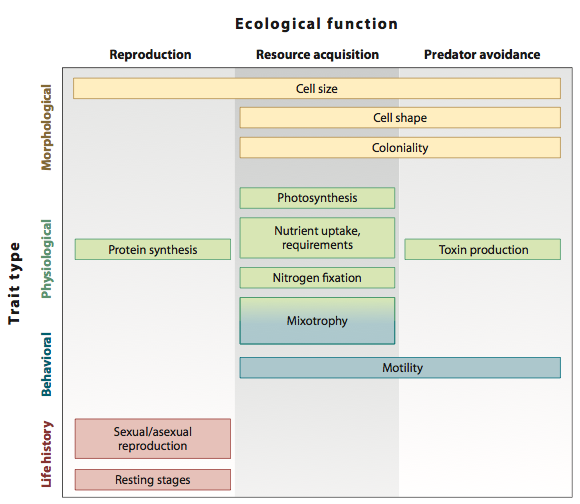
\includegraphics[width=0.7\linewidth]{./Chp1-Intro/Fig_litchman2008.png}
\caption[Scheme]{\small{"A typology of phytoplankton functional traits" from \cite{Litchman2008}}} %have to rewrite in own words!
\label{PhytoTraits}
\end{figure}

{\textbf{Functional types, traits and diversity}}


In the following I will try to clarify the complementary terms
% it is hard to depict this terms as complementary at this point since no definition of trait, functional trait, and functional type have been given
of phytoplankton traits, functional traits, and functional types. 

The trait-based approach to phytoplankton ecology has been growing in popularity. Part of the fascination evoked by this term stems from its origin in evolutionarily theory. Over the last three decades, it has been adopted by ecologists trying to understand communities and ecosystems. In this new context, the concept of traits has been stretched far beyond its original meaning,
% say this after definition or not at all, confusing here
 which can lead to some confusion surrounding the scope of trait-based methods \citep{Violle2007c}. In the simplest definition, a trait is a surrogate of organismal performance. In the ecological context this has been expanded to surrogates for the performance of populations, communities and entire ecosystems. This can include ecophysiological traits, life-history traits, demographic traits or response and effect traits of ecosystems (see Figure \ref{PhytoTraits} for a selection of phytoplankton traits).
 % what are this traits? particularly the last two? you could provide examples to illustrate better the classification of traits.
  Theoretically, any property of an organism or ecosystem could be defined as a trait, but ideally a trait should be functional. 
  % Why a propriety of an ecosystem? and how this squares with McGill definition of a trait, which focus more of trait being a property measured at the individual level?
  Functional traits are defined by \cite{Violle2007c} as "morpho-, physio- or phenological traits which impact fitness indirectly via their effects on growth, reproduction and survival". 
  % could you illustrate this with examples?
   An important facet of the trait-based approach is to describe organismal function via trade-offs between traits. For example when competing for multiple nutrients, phytoplankton species are thought to be constrained by trade-offs in their competitive ability for one over another resource \citep{Tilman1990}. 
   % this a an extremely brief description of what a trade-off is and should be expanded, particularly also read Enquist article of trait-driver theory, and the earlier articles of Jon Norberg on phenotipic traits (PNAS) and on plankton biodiversity (L&O)

Phytoplankton are extremely diverse 
% you have said this several time already without being really precise on what you mean by diversity
and the trait based approach lends itself to generalizations, 
% how? just by defining traits and trade-offs like you suggest afterwards?
as traits and ecological trade-offs can be defined and explored irrespective of species or taxa boundaries \citep{McGill2006}. 
% give examples!
However, depending on the study and hypotheses to be tested, it can be very helpful to structure the diversity of organisms into distinct groups. Major taxonomic groups of phytoplankton can be classified based on their ecological or biogeochemical roles within the ecosystem \citep{Iglesias-Rodriguez2002,Flynn2015}. The concept of functional groups is not in contrast to a trait-based perspective of phytoplankton ecology, but can be complementary to it. By broadly sampling relevant traits across phytoplankton groups and species, functional types can be defined by functional traits and trade-offs and therefore extend the trait-based approach by another level of organization \citep{Litchman2007d}. An early example is the work of Ramón Margalef. Margalef used observations of important traits, such as sinking rates and nutrient utilization to build the concept called "Margalef's mandala" to organize phytoplankton functional types (PFTs) on a spectrum of nutrient availability versus turbulence \citep{Margalef1978}. 

The terms functional group and functional type are used interchangeably, with functional groups more often referring to the grouping of species and the functional type describing the group as a whole, often as implemented in computational models. In fact, the simplification of the phytoplankton community into functional types has been widely used for the design and interpretation of computational models that try to recreate or make predictions about the biogeochemical cycling, biogeographic distribution, productivity and other ecosystem functions of phytoplankton \citep{Gregg2003,LeQuere2005}. Biogeochemically defined functional types are most often used, as these functional traits can usually be well defined within an ecosystem model. Typical examples of such functional groups are silicifers, which broadly correspond the phylogenetic group of diatoms, and calcifiers, which are usually represented by coccolithophores. Such functional types are always simplifications of the natural pyhtoplankton diversity. Silicoflagellates create silicified skeletons like diatoms, but are often not explicitly included because they rarely dominate modern phytoplankton assemblages. The choice of which functional groups to include in a model can also be driven by biogeography or analytical considerations concerning the measurement instrumentation used for a particular study \citep{IrwinAndrewJ.Finkel2017b}.
 % THe PFT part is better explained than the trai part but perhaps you could consider to show it first, since it is a more stablished and better known line of research.  Also consider to use more references to substantiate more your arguments.
 
% And after PFTs you jump into the biodiversity wagon, but still i found it very poorly delivered. I think you proposal would greatly benefit by having a whole section biodiversity, then you could look deeper into the literature about this topic and present a more compelling argument
In biodiversity research, the trait-based approach has been readily adopted. It used to be that species diversity (i.e. the number of species) was the most important metric, but now it is functional diversity, which can be described by the variance in the value of a functional trait of the community or ecosystem. It is important to keep in mind that functional types are often composed of many species with a possibly large variance in trait values. Recent research is trying to understand the effects of diversity within functional types and within species \citep{Violle2012,Violle2017a,DesRoches2018}.
% again this is very brief and reads more like name droping. If you want to talk about intraspecific trait variability then do so but in more detailed manner.




\section{Modeling phytoplankton communities}
Given the complexity of the ocean ecosystem, it is necessary to aggregate our knowledge of the many smaller parts into comprehensive ecological models in order to test mechanistic hypotheses
% EST: what is meant by mechanistic hypotheses?
 and investigate their full-scale implications. Computational models of phytoplankton growth have been developed since the 1940s and have greatly increased in sophistication and complexity since then, co-evolving with the rise in computational resources \citep{Gentleman2002a}. 
 % This is a nice and well referenced opening statement. The rest of the document would greatly benefit from adopting such a style. Hence, if possible consider to eliminate your first sentence, which is not saying much and also try to use more references (either classical works or reviews) in your opening statements. I think it set nicely the stage for what you want to talk about.  
 Phytoplankton modeling started with formulations based on the Lotka-Volterra equations of predator-prey dynamics \citep{Fleming1939}. From these relatively simple descriptions models evolved to describe the oceanic physical environment and the ecosystem it contains including multiple trophic levels. 
 %this needs references to illustrate better
 The nutrient-phytoplankton-zooplankton (NPZ) and nutrient-phytoplankton-zooplankton-detritus (NPZD) models, originally developed by John Steele with a model ocean split in two layers, succeeded in reproducing the typical annual bloom dynamics observed in the temperate ocean \citep{Steele1958,Evans1988,Fasham1990a}. Further developments have been in more exact physiological descriptions of phytoplankton based in cellular metabolism and energy allocation \citep{Geider1997} and both simple and more complicated ecosystem formulations driven by local and global 3D circulation models \citep{Lacroix2007, Hirata2013}.

However, in their simplified approach, these models unavoidably limit the characterization of a diverse phytoplankton community \citep{Bruggeman2009}.
% instead of Jorn's  thesis why not using Follows & Dutkiewicz 2011?
 These plankton ecosystem models are typically highly aggregated, such that a single variable determines the response of a diverse assemblage of phytoplankton species \citep{Franks2009}. Implementing a meaningful treatment of biodiversity in ecological models is a key challenge in the field of phytoplankton modeling \citep{Queiros2015}. The most apparent way of implementing this within the framework of established NPZD models is to include multiple equations and state variables for different phytoplankton functional types \citep{LeQuere2005}. For every group that fulfills a distinct ecosystem function, a new set of parameters has to be added, which complicates the model structure and increases computational costs. This somewhat intuitive approach, however, does lead to problems. First and foremost, there is a lack and inherent uncertainty of data from field and culture experiments to constrain functional types, which leads to the difficulty of validating the model output in light of insufficient information, leading multiple authors to criticize the PFT modeling approach as attempting to "run before we can walk" particularly when used for extrapolating into the future \citep{Anderson2005,Shimoda2016}. 
 % EST: Consider to expand more on Tom Anderson "run before we can walk" paper

The current scientific discussion can seem intimidating to an early career scientist, as both the most obvious future directions of ecosystem model design as exemplified by PFT models, as well as very basic assumptions, such as using Monod nutrient uptake kinetics in phytoplankton models, have come under scrutiny \citep{Flynn2010, Smith2014, Hellweger2017a}.

% EST: Al models have assumptions and limitations. Thus, i do not think previous models are backward looking and that IBM's are forward looking. Eventually IBM's will also hit a wall and something else could come along. Consider to refrain yourself to make such judgments that seem to come out the blue for the reader. If you want to make  comparison between different method you need to elaborate your text with aim from the beginging to list, describe, and explain the different modelling methods and their differences.

Nevertheless, there are also examples of modeling approaches that show a way forward. To name an alternative to the modeling paradigm discussed so far, there is individual based modeling (IBM). In IBM the phytoplankton are explicitly represented as individual agents, allowing for a diverse and spatially interactive phytoplankton community \citep{Hellweger2009}. However, the computational cost and structural complexity of this approach makes both model construction and interpretation difficult. 

Another approach is to extend traditional NPZD models via moment-based estimation of aggregate properties \citep{Merico2009}.
% EST: here you need to cite and read, Wirtz and Eckard 1996, Norberg et al. 2001 and Bruggeman and Kojiman 2007, Yoshiyama 2009
A specific implementation of this is the PhytoSFDM model developed by \citet{Acevedo-Trejos2016}. 
% please refrain to cite me if it is not adding any new and particularly relevant information. Alternatively, If you want to make a delve into different models that have used a moment based estimation then cite them all and breifly explain them.
Instead of modeling multiple size-classes of phytoplankton explicitly, 
% now you are talking about size and size-based models without any background information, please explain and make a logical connection between the topic you want to talk about.
the community is described not only by the biomass, but also by the mean size and size variance. Size is used as a master trait, with size variance being used as a proxy for functional diversity. Trade-offs related to nutrient uptake, grazing and sinking structure the phytoplankton community along the size spectrum as driven by the physical forcing. The model was used to investigate latitudinal diversity gradients in the Atlantic Ocean \citep{Acevedo-Trejos2018}. This approach allows a relatively simple model structure and is computationally efficent, but the PhytoSFDM model structure currently only allows for a single phytoplankton community with a log-normal distribution in cell size. This lends the PhytoSFDM model more to studies of large scale processes and biogeographic patterns rather than to local ecosystem modeling studies, where a more fine-scaled resolution of the phytoplankton community might be required.
% since you are not using a model of aggregate properties i do not see how explaining and going into details of this model helps to make your case. Consider to delete this part all togeteher and only to focus on the the description of the type of models that form the basis for your model, and explain them in detail, i.e. NPZD, PFTs and DARWIN model. 

A major advancement in the field of phytoplankton modeling was the DARWIN model developed at MIT \citep{Follows2007d}. In the general framework of the DARWIN model, large numbers of phytoplankton types are initialized with equal biomass but with different parameters for the most important traits, namely those related to light harvesting, temperature dependence, and nutrient acquisition. These parameters are chosen stochastically from broad ranges of values, based on laboratory and field data, and constrained by simplified allometric functions describing ecological trade-offs. Different functional types are prescribed in the model via varying nutrient utilization traits (e.g. small phytoplankton that cannot assimilate nitrate as Prochlorococcus analogs). Over multi-annual runs this community self-assembles through ecological competition and physical changes produced by the simulated environment of a global circulation model (GCM). In the random initialization of phytoplankton types, the DARWIN model allows for the emergence and development of diverse phytoplankton communities. This approach of modeling biodiversity has been termed “selection-based” \citep{Follows2011c}. 
% explain why selection-based not just mentioned and what other types exist. I think you should use better the references particularly this one
The model framework is continually modified and expanded, for example for exploring the effect of grazing formulations \citep{Prowe2012c}, the biogeography of phytoplankton traits \citep{Barton2013} and the influence of ocean acidification at a global scale \citep{Dutkiewicz2015}. A study of particular interest is the size-structured food-web model component developed by \citet{Ward2012}, because the modeling approach combines the trait-based approach of scaling parameters allometrically along cell size with a PFT modeling approach. 
% why is this particularly interesting and why size and size based model? Are you going to develop a size based model?
Each functional type is assigned a different allometry based on the size ranges and relationships taken from data. Together with the selection-based biodiversity representation that the DARWIN framework provides, this seems to be a promising direction for future models. The model has however only been applied and compared to data at a global scale and the code of this specific implementation is not publicly available. 

% why there should be a consensus on the most promising tools in the first place? and how one reach that?
The field of phytoplankton modeling provides diverse approaches and no consensus has been reached as to which computational tools and model structures are the most promising. In describing an ecosystem in computational models, a balance needs to be found between complexity and simplicity. The natural ecosystems are invariably very complex, however models that capture too much of the detail are difficult to interpret, and overtly simplistic models risk not capturing the essential dynamics present. Another important aspect of model development, no matter where it lies on the scale of complexity, is model validation using ecological data \citep{RykielJr1996}. In fact model complexity might generally have to be adapted to the scientific question at hand, which often emerges from patterns observed in ecological data. 
% the conclusion of this subsection it is fairly shallow and repetitive. Thus consider to rewrite it.


\section{The Cariaco Basin and the CARIACO time-series}
\label{CARIACOintro}

%need to explain SST somewhere! im using it later a lot

At the beginning of my PhD I set out to find publicly available ocean time-series data that could be used as the basis for modeling work about phytoplankton diversity. Initially the plan was to choose multiple locations, to compare results from model applications in contrasting environments. Not surprisingly the search did quickly yield results, among the most prominent: the Bermuda Atlantic Time-series Study (BATS) and the Hawaii Ocean Time-Series (HOTS). Quickly the issues of public ocean time-series data became apparent. Links often lead to defunct sites and servers were sporadically maintained. In particular for my application the problem was that the basic physical parameters and bulk properties such as total chlorophyll were readily available, but more specific phytoplankton functional type or taxonomy data was harder to find, if not missing. In particular the type of phytoplankton data that was available differed widely between the stations and would have not allowed for a straightforward comparison. It was only later in my search that I came across the CARIACO time series, 
% consider to delete this part since it does not provide any useful information to better understand the CARIACO time series data
an acronym for "CArbon Retention In A Colored Ocean", located in the Cariaco Basin off the coast of Venezuela. The data is available through the University of South Florida (USF) at \href{http://imars.marine.usf.edu/cariaco}{http://imars.marine.usf.edu/cariaco} and includes a wealth of data that was collected since 1995. Most importantly to my purposes, the data included both detailed phytoplankton pigment measurements and taxonomic data of the phytoplankton community at monthly intervals. It was the first ocean time-series with such detailed public phytoplankton data and soon I decided to focus my work on the Cariaco Basin. Previous work specifically using the phytoplankton dataset has to my knowledge been limited to statistical modeling and analysis \citep{Taylor2012,Mutshinda2013a, Mutshinda2013,Pinckney2015,Irwin2015}. Apart from an early study looking at carbon fluxes, where the only resolved functional type in the ecosystem model were diatoms \citep{Walsh2002a}, there has been no study using a mechanistic ecosystem model applied to the CARIACO time-series, allowing for novel applications and insights from my PhD thesis.
% avoid this type of informal statements in the introduction and better point out the scientific gaps    

The CARIACO time-series station has historically been a site of scientific interest and served as a natural laboratory in biogeochemical research for more than 60 years \citep{Muller-Karger2019a}. It has played important roles in understanding the nutrient stoichiometry of the ocean \citep{Redfield1963}. The CARIACO Ocean Time-Series program was established in 1995 off the coast of Venezuela (10$^\circ$ 30$'$ N, 64$^\circ$ 40$'$ W, see Figure \ref{CARIACO-map}). Located in the south-eastern Caribbean Sea, the Cariaco Basin is a 160 km long and 70 km wide tectonic depression, reaching up to 1400 m in depth. The two deeper parts of the basin are separated by a saddle of 900 m depth, with the time-series mooring located in the eastern part. The entire basin is bound to the west and north by a shallow ridge at 100 m depth, restricting the exchange of deep water with the Caribbean Sea. The restricted circulation and high productivity at the surface resulted in anoxic conditions below 250 m depth within the basin \citep{Richards1956}. The Cariaco Basin is the worlds largest truly marine anoxic basin \citep{Wakeham2012}. The hydrography at the surface is influenced by Guyana and North Equatorial currents that flow into the Caribbean Sea from a south-eastern direction, but this exchange is restricted to the two channels above the 100 m ridge. Observed and modeled horizontal surface water velocities within the basin are relatively weak, indicating a minimal influence of horizontal transport at the mooring site \citep{Alvera-Azcarate2009}. 

\begin{figure}
\centering
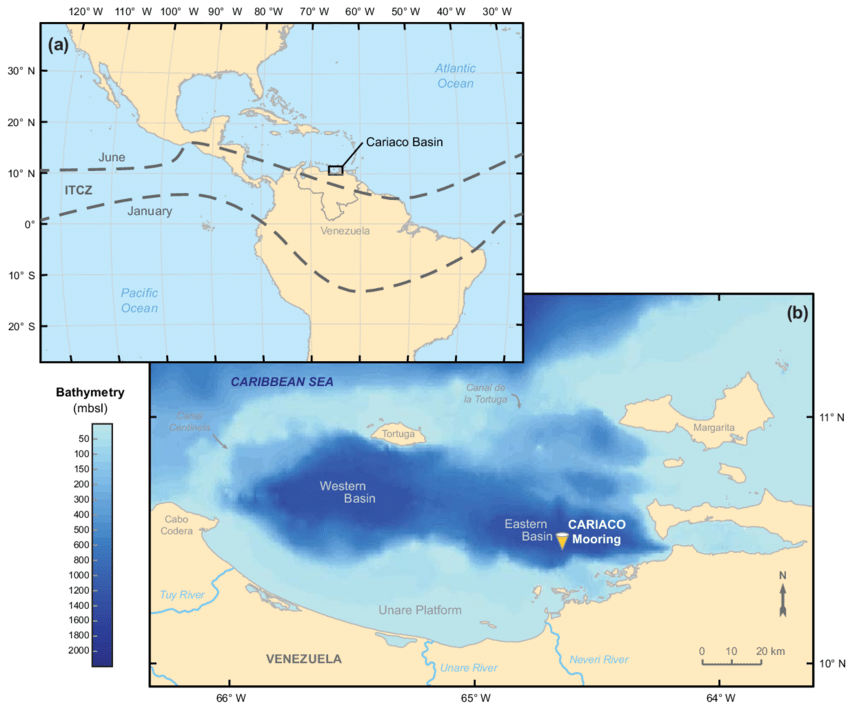
\includegraphics[trim = 0mm 0mm 0mm 0mm, clip, width=1.\linewidth]{./Chp1-Intro/CARIACObasinMAP_Bringueetal2018.png}
\caption[Scheme]{\small {"Study area. A. Location of the Cariaco Basin off the Venezuelan coast in the southern Caribbean Sea, with January and June positions of the Intertropical Convergence Zone (ITCZ). B. Location of the CARIACO station in the eastern sub-basin, general bathymetry and local rivers emptying in the basin (bathymetric data from GEBCO\_08 Grid)" from \cite{Bringue2019}}} % % EST: see comments to figure 1.1 and why you did not produce your own map?
\label{CARIACO-map}
\end{figure}



{\textbf{The time-series data}}

The program was established as a joint-project of the Venezuelan Fondo Nacional de Cienca, Tecnolog\'{i}a e Investigac\'{i}on (FONACIT) and the US National Science Foundation (NSF), with the particular interest in creating a time-series of surface ocean biogeochemistry that could be linked to satellite observations and the sedimentation accumulating in the anoxic basin. 
% this read a bit repetitive try to be more concise
Since  November 1995 there were 232 core cruises at mostly monthly intervals, in addition to sediment trap and microbial-biogeochemistry process cruises. The full set of measurements and determination methods taken can be found in the manual of methods that was published by the coordinators of the time-series \citep{Astor2013}. 
% if the information you provide is not helping you to build your argument then please refrain to used. Just listing all the information about the time series is
Of particular interest to my applications are the detailed nutrient measurements 
% to this point the reader does not know what are you going to do, you haven't out line the aims or research questions you want to tackle so how can a reader follow you line of reasoning that this is relevant to your study? 
% Please refrain to just present the relevant data to your study without making this type of informal judgments without providing the reader with context to make their own judgment
taken using a Niskin bottle sampler and continous flow analysis (see Figure \ref{CARIACOnuts} for contour plots of Nitrate, Phosphate and Silicate), as well as the phytoplankton taxonomy (see Figure \ref{PFTcariaco} for PFT abundances) and high-pressure liquid chromatography (HPLC) measurements (see Figure \ref{TChlAPinckney} for HPLC derived total chlorophyll a $chl~a$) also taken at discrete depth intervals over the duration of the time series. 

\begin{figure}
\centering
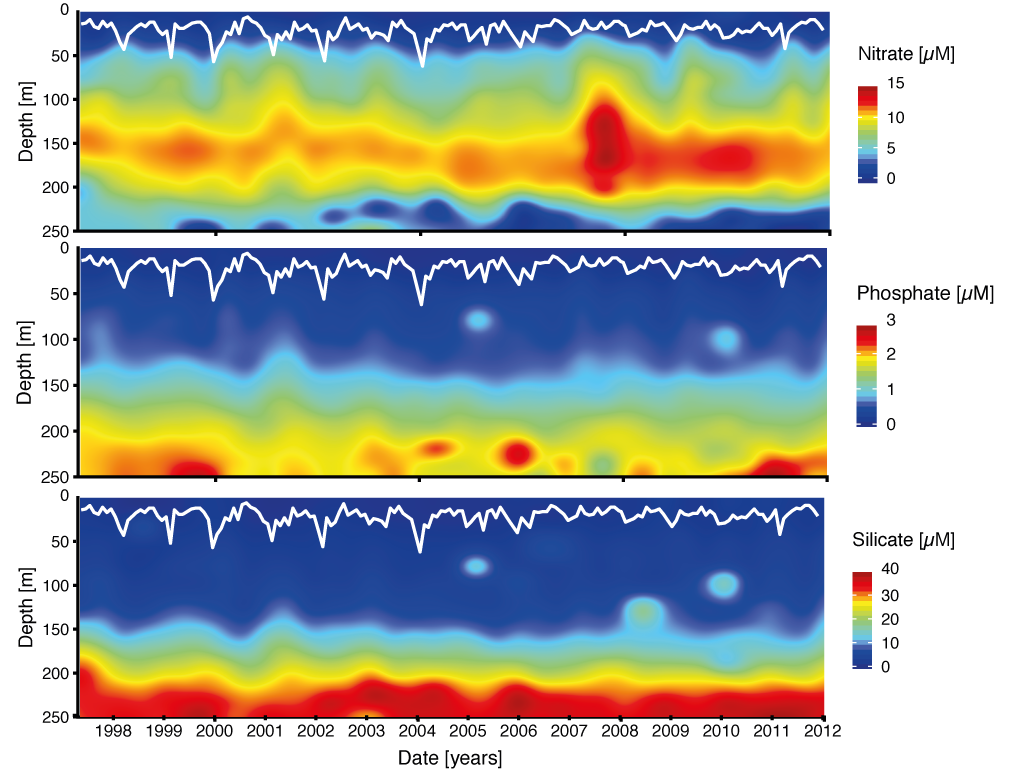
\includegraphics[trim = 0mm 0mm 0mm 0mm, clip, width=1.\linewidth]{./Chp1-Intro/NUTSatCARIACOAsset811.png}
\caption[Scheme]{\small {Contour plots of Nitrate, Phosphate and Silicate of the CARIACO time series down to 250 m. White line shows depth of MLD.}} 
\label{CARIACOnuts}
\end{figure}

The general dynamics observed over the course of the time-series are comprehensively discussed in a recent review paper by \citet{Muller-Karger2019a}. 
% Consider to rather than spend so many words to cite an article to just describe the patterns in the data and then just cite the relevant literature.
In the same publication it was also announced that the time-series was officially ended, due to a lack of funding. However, in the two decades that it existed the time-series data created a detailed description of the biogeochemistry of the Cariaco Basin. Despite the tropical location of the time series, the data reveals a seasonal cycle driven by upwelling along the southern coastline of the Caribbean Sea occuring usually between November and August, as trade winds intensify with the southward migration of the Intertropical Convergence Zone (ICTZ) 
% Please expend a few word explaining what the ITCZ is
(see Figure \ref{CARIACO-map}, A). The influx of nutrients provides the basis for high productivity (320 to 628 g C m$^{-2}$ y$^{-1}$) in the surface waters of the basin. This drives vertical export, with 9 to 10 g C m$^{-2}$ y$^{-1}$ reaching the bottom sediments, which amounts to 1-3 \% of primary production (PP) \citep{Muller-Karger2019a}. The waters are inhabited by a diverse community of microorganism, in particular at the oxic-anoxic interface at roughly 250 m depth where novel eukaryotes have been found \citep{Stoeck2003}. 
% why mention novel organisms and not provide any extra information. Is it relevant to mention that to make your point? and what is exactly the point you want to make in this paragraph? 


\begin{figure}
\centering
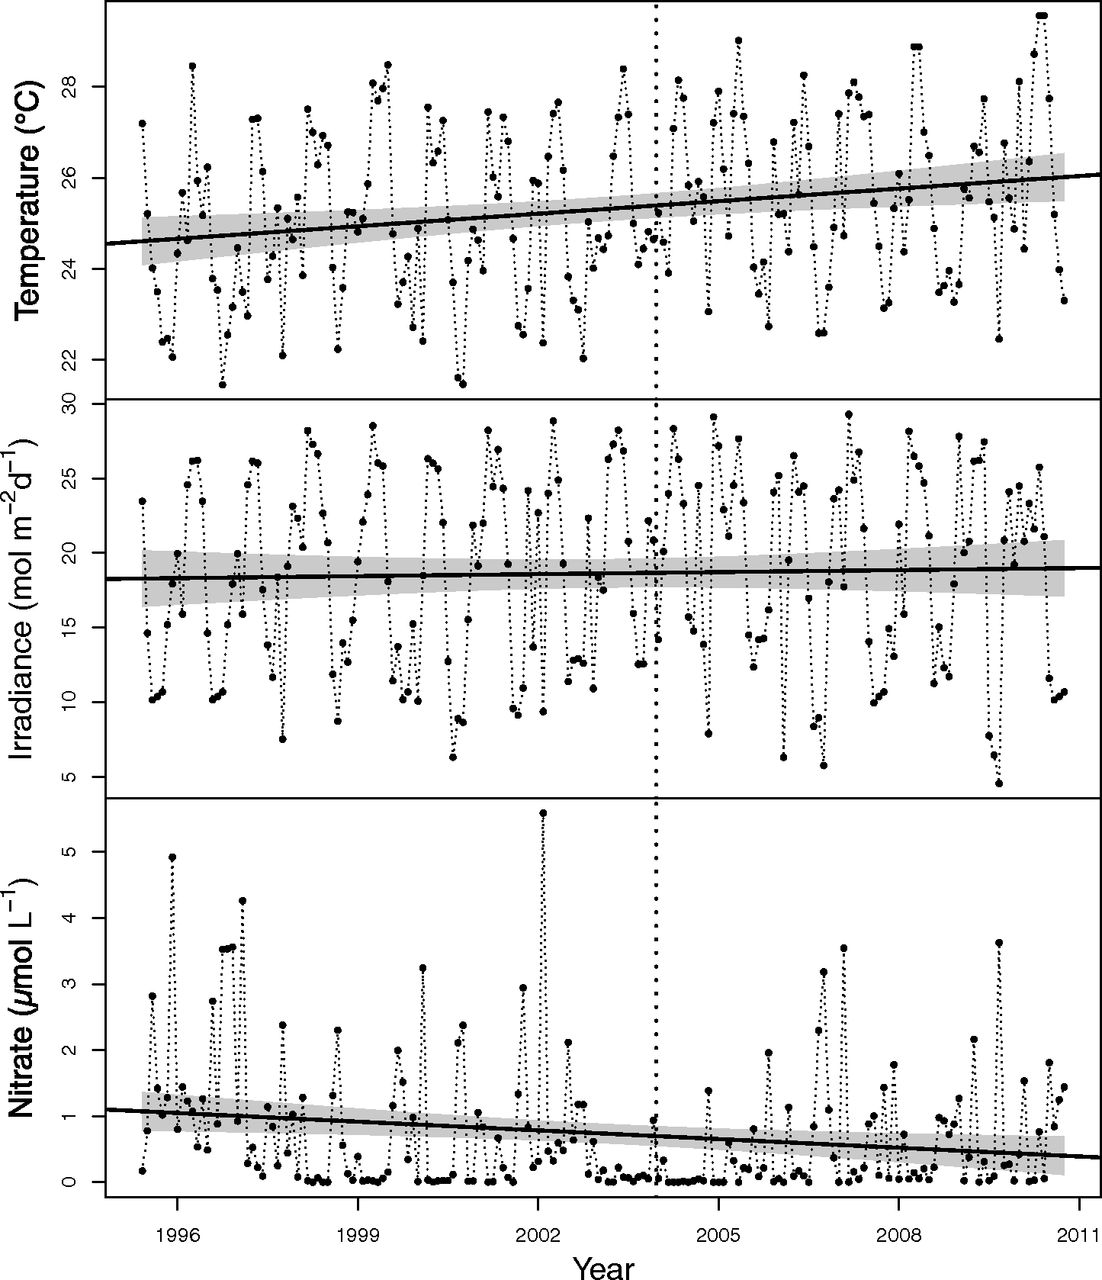
\includegraphics[trim = 0mm 0mm 0mm 0mm, clip, width=0.7\linewidth]{./Chp1-Intro/IRWIN_F1.large.jpg}
\caption[Scheme]{\small {"Monthly environmental conditions averaged over the upper mixed layer (1, 7, 15, and 25 m depth) from the CARIACO Ocean Time-Series Program: temperature ($^\circ$C), irradiance (mol m$^{–2}$ d$^{–1}$), and nitrate concentration ($\mu$mol L$^{–1}$). The vertical dotted line is drawn at the boundary (January 1, 2004) between the cool and warm periods. The straight lines are linear regressions: temperature = (24.6 $\pm$ 0.3) + (0.09 $\pm$ 0.03)$t$, $R^2$ = 0.05, P \textless 0.005; irradiance = (18.1 $\pm$ 0.9) + (0.05 $\pm$ 0.11)$t$, $R^2$= 0.001, P = 0.65; nitrate = (1.06 $\pm$ 0.14) – (0.045 $\pm$ 0.017)$t$, $R^2$ = 0.04, P = 0.03, where $t$ is time in years since January 1, 1996, errors are one SE, and the shaded region is the 95\% confidence interval on the line. The $R^2$ is very low because of the tremendous interannual variation relative to the trend." from \cite{Irwin2015}}} % EST:  see comments to figure 1.1 and if we have the data why you  did not plot the data yourself?
\label{CARIACOTaylorTrends}
\end{figure}

Long-term trends show a reduction in upwelling intensity in the time from 2003 to 2013, which has been linked to a weakening trend in the trade winds and the north-easterly movement of the Atlantic centroid of the ICTZ 
% how the reader should know what it is the Atlantic centroid of the ITCZ?
\citep{Taylor2012}. This reduction in upwelling is visible in a reduction nitrate concentration and coincides with an increase in temperature across the upper mixed layer (see Figure \ref{CARIACOTaylorTrends}). 
% EST: rephrase the previous sentence!

% it is not clear the period you are referring to here and also consider like is many of the previous paragraphs to not end with a list of facts and try to sumarize or conclude each paragraph so the reader can better understand what is you want to comunicate what is your take home message: 
The change in physical conditions was accompanied by a shift in the biotic community. Phytoplankton bloom intensities were reduced, while phytoplankton diversity and zooplankton densities showed an increasing trend. Interestingly, vertical export remained at a similar level, despite the fact that phytoplankton taxonomy data shows a marked reduction in larger phytoplankton species. \citep{Taylor2012,Pinckney2015}. The increase in zooplankton densities was linked to a collapse in the local sardine fisheries (see Figure \ref{TaylorSHIFTS}). The biogeochemistry of the deeper waters reflects a shift in the biotic community at the surface \citep{Scranton2014}. 

\newpage
\section{Aims of the proposed PhD project}

The marked dynamics captured in the CARIACO time-series provide a wealth of data to explore during my PhD. With the upcoming collaboration with Andrew Barton at the Scripps Institution of Oceanography I will be working under the supervision of a phytoplankton modeling expert who has direct experience of the CARIACO dataset, as he himself worked on a proposal for an ecosystem modeling study in the region that was unfortunately not funded. I am also in contact with James Pinckney and Claudia Benitez-Nelson from the University of South Carolina, who have been heavily involved in the scientific project of CARIACO and have been kind enough to share specific datasets that were not publicly available. The general aim of my PhD Project, as exemplified by the three planned manuscripts, is to build a framework to explore the shifts observed in the phytoplankton community in the Cariaco Basin.
% building a framework is not an aim of PhD project in ecology. Can you formulate a general aim in the form of a general scientific question relevant to your work?

% Your general objective should not be depend on the availability of data or the plausibility to work with Andrew or because you are in contact with a scientist by email.  This reads very poorly and have to be amended. Please consider to better highlight an overall scientific question 

\begin{itemize}
\item The first study will focus on the biomass dynamics observed in the HPLC-derived phytoplankton pigment data. I have built an ecosystem model that resolves multiple nutrients and multiple functional types of both phytoplankton and zooplankton. The goal is to explore the drivers of community composition. Hypothesis of bottom-up and top-down processes (a decrease in upwelling and an increase in zooplankton grazing respectively) driving these changes have been put forward in the literature. The ecosystem model would allow for a mechanistic exploration of the effects of these processes on the phytoplankton community, with a direct comparison to the dynamics observed in the CARIACO data. % similar to my previous comment it is not clear what is scientific question you want to address here also it did not helped that in the introduction no open questions where highlighted.
\item During the model construction of the first study, I developed a technical concept to implement a flexible PFT model framework in the open-source programing language Python. The code structure allows for any combination and amount of functional types to be added to the model structure, which lends itself very well to the study of biodiversity effects, as well as simply implementing different types of ecosystem models. This structure is already used within the first study, however I aim to fully develop the code as a Python package, to release to the scientific community. The python package will form the basis of a technical manuscript to be submitted to the journal Geoscientific Model Development. % Since this is your main tool during your phd studies, then try to formulate the specific scientific aim in line with the general aim / question
\item As the first study uses a PFT modeling approach, but otherwise does not explore the effects of biodiversity on ecosystem function, the third study will aim to address this issue with the help of the  developed modeling tool. The CARIACO time-series provides a rich dataset to test hypotheses, in particular of the effects of intra- and inter-PFT diversity. The collaboration with Andrew Barton is central to the formulation the specific scientific questions and model implementations. I aim to complete this project in the third year of my PhD. % again the specific aim should be inspired the by the general scientific question / aim and would greatly benefit to also tackle a pressing scientific question in BEF research. Read Brose and Hillebrand 2016 and some of the article in that special issue for inspiration as well as Michele Loreau classical works on the topic (1999 PNAS, 2001 Nature). 
\end{itemize}
